\documentclass[tikz,border=10pt]{standalone}
\usetikzlibrary{intersections}
\let\phi\varphi
\begin{document}
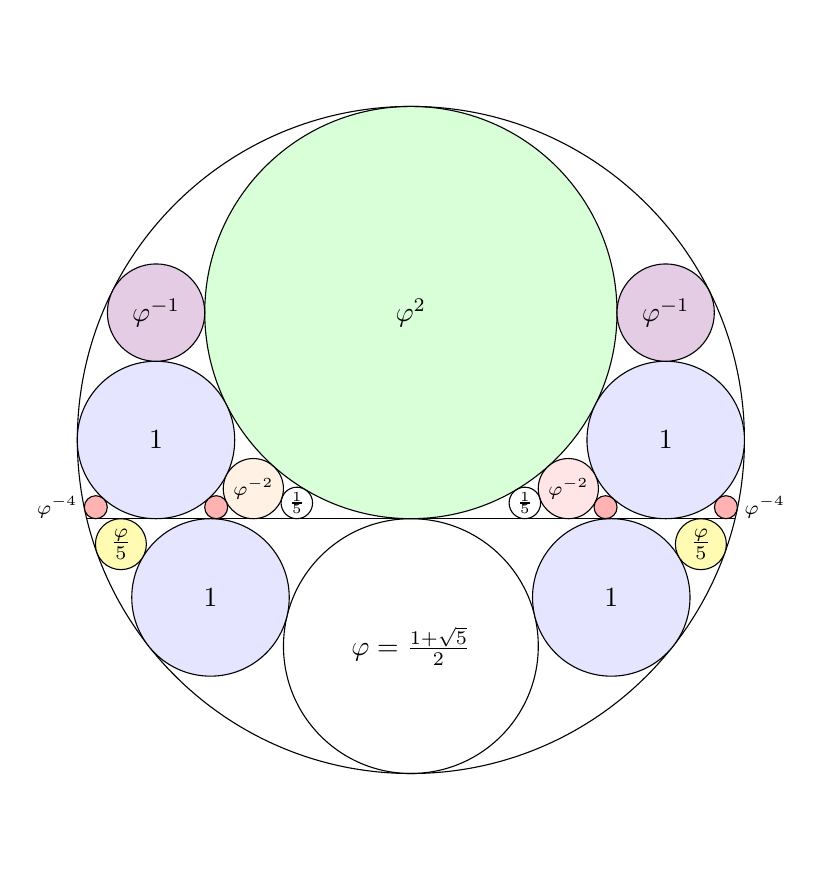
\begin{tikzpicture}[nodes = {execute at begin node=$, execute at end node=$}]
  \pgfmathsetmacro\r{(1+sqrt(5))/2}
  \draw [name path=c1] circle(\r) node{\phi=\frac{1+\sqrt{5}}{2}};
  \draw [name path=c2,fill=green!15] (0,\r+\r^2) circle(\r^2)  node{\phi^2};
  \draw [name path=c3] (0,\r^3-\r) circle(\r^3);
  \path [name path=l] (-\r^3,\r) -- (\r^3,\r);
  \draw [name intersections={of=l and c3, name=l0}] 
        (l0-1) -- (l0-2);

  \path [name path=l1] (-\r^3,\r+1) -- (\r^3,\r+1);
  \path [name path=c4] (0,\r+\r^2) circle(\r^2+1);
  \draw [name intersections={of=l1 and c4, name=c},fill=blue!10] 
        (c-1) circle (1) node {1};
  \draw [fill=blue!10] (c-2) circle (1) node {1};

  \path [name path=l4] (-\r^3,\r-1) -- (\r^3,\r-1);
  \path [name path=c8] (0,0) circle(\r+1);
  \draw [name intersections={of=l4 and c8, name=c9},fill=blue!10] 
        (c9-1) circle (1) node {1};
  \draw [name intersections={of=l4 and c8, name=c9},fill=blue!10] 
        (c9-2) circle (1) node {1};

  \path [name path=c5] (0,\r+\r^2) circle(\r^2+\r^-2);
  \path [name path=l2] (-\r^3,\r+\r^-2) -- (\r^3,\r+\r^-2);
  \draw [name intersections={of=l2 and c5, name=c6},fill=orange!10] 
        (c6-1) circle (\r^-2) node [font=\scriptsize] {\phi^{-2}};
  \draw [fill=red!10] (c6-2) circle (\r^-2) node [font=\scriptsize] {\phi^{-2}};

  \path [name path=c7,dotted] (0,\r+\r^2) circle(\r^2+1/5);
  \path [dotted,name path=l3] (-\r^3,\r+1/5) -- (\r^3,\r+1/5);
  \draw [name intersections={of=l3 and c7, name=c8}] 
        (c8-1) circle (1/5) node[font=\tiny] {\frac{1}{5}};
  \draw [] (c8-2) circle (1/5) node[font=\tiny] {\frac{1}{5}};

  \path [name path=l5] (-\r^3,\r-\r/5) -- (\r^3,\r-\r/5);
  \path [name path=c10] (c9-1) circle(1+\r/5);
  \draw [name intersections={of=l5 and c10, name=c11},fill=yellow!30] 
        (c11-1) circle (\r/5) node {\frac{\phi}{5}};
  \path [name path=c12] (c9-2) circle(1+\r/5);
  \draw [name intersections={of=l5 and c12, name=c13},fill=yellow!30] 
        (c13-2) circle (\r/5) node {\frac{\phi}{5}};

  \path [name path=c16] (0,\r+\r^2) circle(\r^2+\r^-1);
  \path [name path=c14] (c-1) circle(1+\r^-1);
  \draw [name intersections={of=c14 and c16, name=c15},fill=violet!20] 
        (c15-1) circle (\r^-1) node {\phi^{-1}};
  \path [name path=c16] (0,\r+\r^2) circle(\r^2+\r^-1);
  \path [name path=c17] (c-2) circle(1+\r^-1);
  \draw [name intersections={of=c17 and c16, name=c18},fill=violet!20] 
        (c18-1) circle (\r^-1) node {\phi^{-1}};

  \path [name path=l6] (-\r^3,\r+\r^-4) -- (\r^3,\r+\r^-4);
  \path [name path=c19] (c-1) circle(1+\r^-4);
  \draw [name intersections={of=l6 and c19, name=c20},fill=red!30] 
        (c20-1) circle (\r^-4) node[font=\scriptsize,xshift=-14] {\phi^{-4}};
  \draw [fill=red!30] 
        (c20-2) circle (\r^-4);

  \path [name path=c21] (c-2) circle(1+\r^-4);
  \draw [name intersections={of=l6 and c21, name=c22},fill=red!30] 
        (c22-2) circle (\r^-4) node[font=\scriptsize,xshift=14] {\phi^{-4}};
  \draw [fill=red!30] 
        (c22-1) circle (\r^-4);
\end{tikzpicture}
\end{document}